\documentclass{article}
\usepackage{amsfonts}
\usepackage{amsmath}
\usepackage{listings}
\usepackage{mybigpackage}
\usepackage{graphicx}

\begin{document}
	\title{\textbf{Assignment-10}}
	\author{Abheek Ghosh \\ 
		140123047 }
	
	\maketitle
	

\section{Question 1}

\noindent{Code for R}

\begin{lstlisting}
m <- 500 # No. of paths
n <- 5000  # No of time points
k <- 0

# Time
t <- 5
dt <- t/n

# Properties of Stock selected by us
s0 <- 100   # initial price
Mu <- c(-0.1, 0.05, 0.1)
Sigma <- c(0.01, 0.02, 0.03)

# Some required extras
w5 <- vector(,m)
T <- seq(0, t, dt)
pal <- palette()

for (mu in Mu) {
    for (sigma in Sigma) {

        for (i in 1:m) {
            Z <- rnorm(n)
            S <- cumsum(c(log(s0), (mu - (sigma^2)/2)*dt + sigma*(dt^(1/2))*Z))
            S <- exp(S)
            w5[i] <- S[n + 1]
            if(i == 1) {
                plot(T, S,  col=pal[i %% 8 + 1], cex=0.00001, main=paste0("Stock price, S(0)=",toString(s0),", mu=",toString(mu)," sigma=",toString(sigma)), xlab="Time", ylab="Stock Value", type="l")
            } else if (i <= 10){
                lines(T, S, col=pal[i %% 8 + 1], cex=0.00001)
            }
        }
        k <- k + 1
        dev.copy(png,paste0("plot",toString(k),".png"));
        dev.off ();

        cat("\nStock price, S(0)=",s0,", mu=",mu," sigma=",sigma,"\\\\\\\\\n")
        cat(" Expected value of S(5), Theoretical = ", s0*exp(mu*t), ", Simulated = ", mean(w5),"\\\\\n")
        cat(" Variance of S(5) Theoretical = ", (s0^2)*(exp(2*mu*t)*(exp((sigma^2)*t) - 1)) , ", Simulated = ", var(w5),"\\\\\n\n")
        cat("\\includegraphics{",paste0("plot",toString(k)),"}\n")
        cat("\\pagebreak \n\n")

    }
}

rm(list = ls())


\end{lstlisting}
Stock price, S(0)= 100 , mu= -0.1  sigma= 0.01 \\\\
 Expected value of S(5), Theoretical =  60.65307 , Simulated =  61.30941 \\
 Variance of S(5) Theoretical =  1.839857 , Simulated =  1.612707 \\

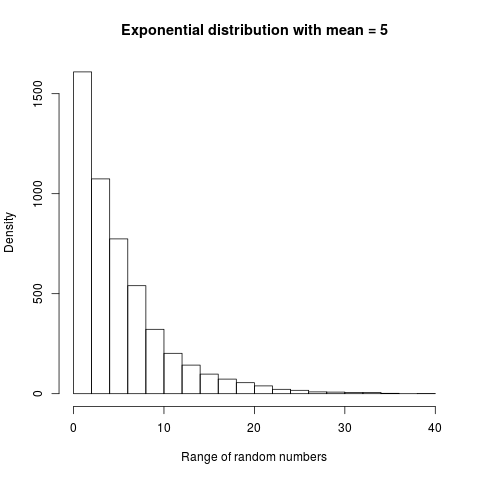
\includegraphics{plot1}
\pagebreak 


Stock price, S(0)= 100 , mu= -0.1  sigma= 0.02 \\\\
 Expected value of S(5), Theoretical =  60.65307 , Simulated =  62.05115 \\
 Variance of S(5) Theoretical =  7.364951 , Simulated =  6.333595 \\

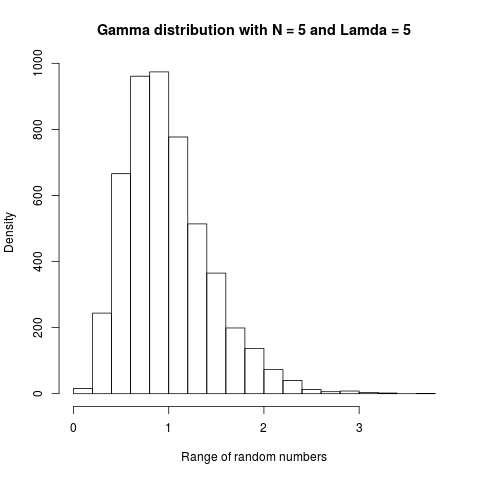
\includegraphics{plot2}
\pagebreak 


Stock price, S(0)= 100 , mu= -0.1  sigma= 0.03 \\\\
 Expected value of S(5), Theoretical =  60.65307 , Simulated =  61.04375 \\
 Variance of S(5) Theoretical =  16.59188 , Simulated =  15.36735 \\

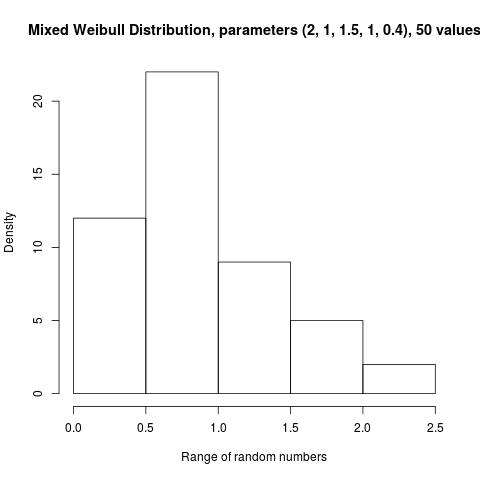
\includegraphics{plot3}
\pagebreak 


Stock price, S(0)= 100 , mu= 0.05  sigma= 0.01 \\\\
 Expected value of S(5), Theoretical =  128.4025 , Simulated =  127.5122 \\
 Variance of S(5) Theoretical =  8.245668 , Simulated =  7.316898 \\


\includegraphics{plot4}
\pagebreak 


Stock price, S(0)= 100 , mu= 0.05  sigma= 0.02 \\\\
 Expected value of S(5), Theoretical =  128.4025 , Simulated =  127.5635 \\
 Variance of S(5) Theoretical =  33.00742 , Simulated =  32.21786 \\

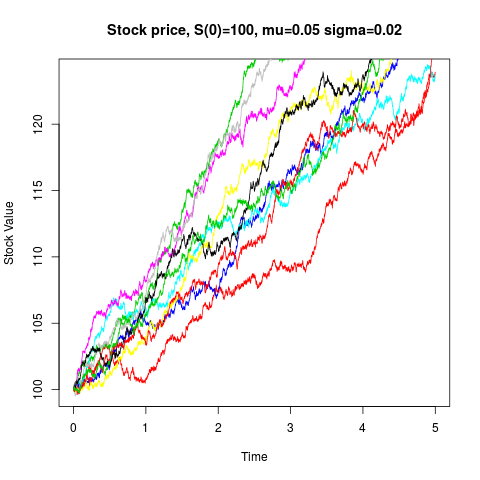
\includegraphics{plot5}
\pagebreak 


Stock price, S(0)= 100 , mu= 0.05  sigma= 0.03 \\\\
 Expected value of S(5), Theoretical =  128.4025 , Simulated =  133.3569 \\
 Variance of S(5) Theoretical =  74.35964 , Simulated =  75.69611 \\

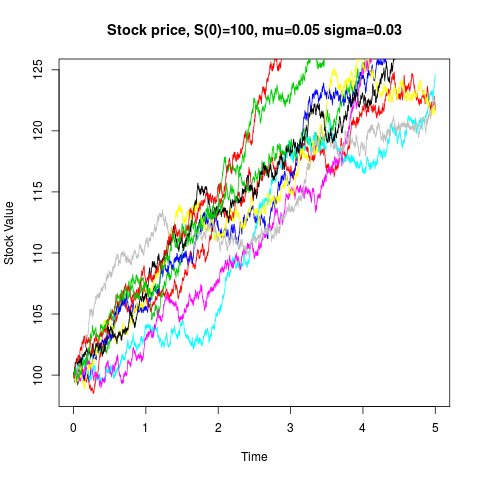
\includegraphics{plot6}
\pagebreak 


Stock price, S(0)= 100 , mu= 0.1  sigma= 0.01 \\\\
 Expected value of S(5), Theoretical =  164.8721 , Simulated =  165.3967 \\
 Variance of S(5) Theoretical =  13.59481 , Simulated =  12.23939 \\

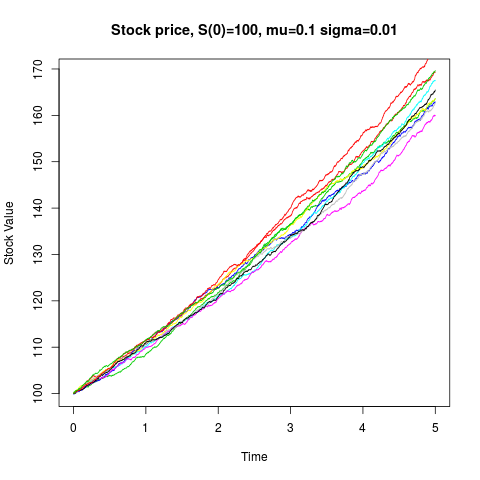
\includegraphics{plot7}
\pagebreak 


Stock price, S(0)= 100 , mu= 0.1  sigma= 0.02 \\\\
 Expected value of S(5), Theoretical =  164.8721 , Simulated =  165.2831 \\
 Variance of S(5) Theoretical =  54.42004 , Simulated =  51.992 \\

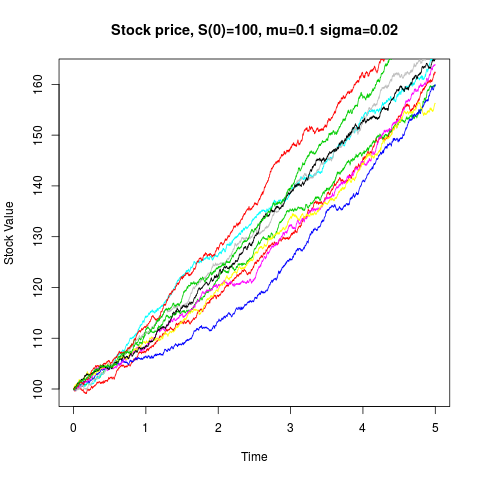
\includegraphics{plot8}
\pagebreak 


Stock price, S(0)= 100 , mu= 0.1  sigma= 0.03 \\\\
 Expected value of S(5), Theoretical =  164.8721 , Simulated =  169.1438 \\
 Variance of S(5) Theoretical =  122.5983 , Simulated =  118.6379 \\

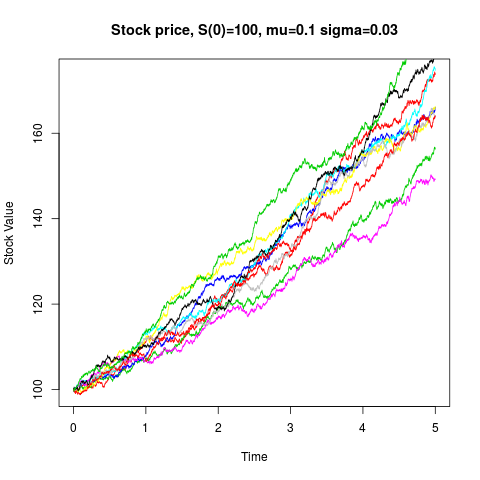
\includegraphics{plot9}
\pagebreak 
\end{document}
